\documentclass[12pt]{article}

\usepackage[latin1]{inputenc}
\usepackage{amssymb}
\usepackage{amsmath}
\usepackage{amsthm}
\usepackage{latexsym} 
\usepackage{graphicx}
\usepackage{bm}  
\usepackage{overpic} 
\usepackage[normalem]{ulem}
  
\usepackage{exscale}
\usepackage{amsfonts}
\usepackage[usenames,dvipsnames]{color} % load color package

\textwidth=6.0in \textheight=8.8in \hoffset=-0.2in
\voffset=-0.85in
\parskip=6pt
\baselineskip=9pt
\topmargin 0.8in
 
\def\black#1{\textcolor{black}{#1}}
\def\blue#1{\textcolor{blue}{#1}}
\def\red#1{\textcolor{red}{#1}}
\def\green#1{\textcolor{green}{#1}}
\def\yellow#1{\textcolor{yellow}{#1}}
\def\orange{\textcolor{BurntOrange}}

\newtheorem{definition}{Definition}[section]
\newtheorem{lemma}{Lemma}[section]
\newtheorem{remark}{Remark}[section]
\newtheorem{example}{Example}[section]
\newtheorem{theorem}{Theorem}[section]
\newtheorem{cor}{Corollary}[section]
\newtheorem{corollary}{Corollary}[section]

\numberwithin{equation}{section}

\newcommand{\E}{\mathbb{E}}
\newcommand{\R}{\mathbb{R}}
\newcommand{\sigl}{\sigma_L}
\newcommand{\BS}{\rm BS}
\newcommand{\p}{\partial}
\newcommand{\var}{{\rm var}}
\newcommand{\cov}{{\rm cov}}
\newcommand{\beaa}{\begin{eqnarray*}}
\newcommand{\eeaa}{\end{eqnarray*}}
\newcommand{\bea}{\begin{eqnarray}}
\newcommand{\eea}{\end{eqnarray}}
\newcommand{\ben}{\begin{enumerate}}
\newcommand{\een}{\end{enumerate}}


\def\cC{\mathcal C}
\def\cD{\mathcal D}
\def\cS{\mathcal S}
\def\cH{\mathcal H}
\def\cI{\mathcal I}
\def\cJ{\mathcal J}
\def\cL{\mathcal L}
\def\cV{\mathcal V}
\def\cR{\mathcal R}
\def\bR{\mathbb R}
\def\cX{\mathcal X}
\def\cF{\mathcal F}
\def\bP{\mathbb P}
\def\bE{\mathbb E}
\def\bN{\mathbb N}
\def\bT{\mathbb T}
\def\bC{\mathbb C}
\def\var{\text{var\,}}
\def\eps{\varepsilon}

\newcommand{\mt}{\mathbf{t}}
\newcommand{\mS}{\mathbf{S}}
\newcommand{\tC}{\widetilde{C}}
\newcommand{\hC}{\widehat{C}}
\newcommand{\tH}{\widetilde{H}}
\renewcommand{\O}{\mathcal{O}}
\newcommand{\dt}{\Delta t}
\newcommand{\tr}{{\rm tr}}

\begin{document}



\title{\bf Our brilliant masters project final report}

\author{John Brown\footnote{Department of Mathematics, Baruch College, CUNY. {\tt  john.brown@baruch.cuny.edu}}{\setcounter{footnote}{1}} , James Smith\footnote{Department of Mathematics, Baruch College, CUNY. {\tt  James.Smith@baruch.cuny.edu}}{\setcounter{footnote}{2}} \thanks{We wish to thank our hamsters Buster and Butch for their constant affection.}
}

%\date{This version: December 25, 2011}


\maketitle\thispagestyle{empty}
 
%%***************************************************************************
%%
%%  Document begins here
%%
%%***************************************************************************



\begin{abstract}
In this report, we describe our final project ....
\end{abstract}

%%%%%%%%%%%%%%%%%%%%%%%%%%%%%%%%%%%%%%%%%%%%%%%%%%%%%%%%%%%%%%%%%%%%%%%%%%%%%%%%%
%
%
%  Section: Introduction
%
%
%%%%%%%%%%%%%%%%%%%%%%%%%%%%%%%%%%%%%%%%%%%%%%%%%%%%%%%%%%%%%%%%%%%%%%%%%%%%%%%%%%

\section{Introduction}



\subsection{Prior literature}


\section{Our main result}

\begin{theorem}\label{thm:GreatTheorem}
For any given positive integer $n$, there exists at least one integer greater than $n$.
\end{theorem}

\begin{proof}
Consider $m=n+1$.     
\end{proof}

\begin{remark} 
Note just how brilliant Theorem \ref{thm:GreatTheorem} is!
\end{remark}

We obtain
\begin{cor}
There exists an integer greater than 3.
\end{cor}

\section{Another result}


\section{Numerical experiment}

\begin{figure}[htb!]
\begin{center}
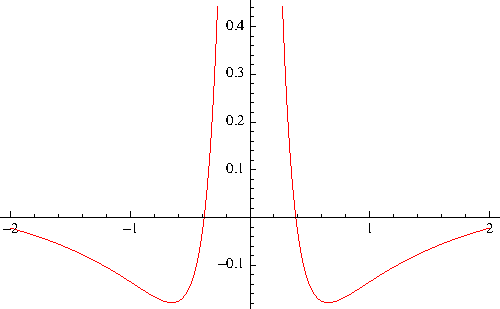
\includegraphics{SVIarb}
\caption{This is a graph of something}
\label{fig:someGraph}
\end{center}
\end{figure}



\section{Summary and conclusion}


%\appendix





\section*{Acknowledgments}

We are very grateful to Jane Brown and Janice Smith.

%%%%%%%%%%%%%%%%%%%%%%%%%%%%%%%%%%%%%%%%%%%%%%%%%%%%%%%%%%%%%%%%%%%%%%%%%%%%%%%%%%%%%%%%
%
%
%  Bibliography
%
%
%%%%%%%%%%%%%%%%%%%%%%%%%%%%%%%%%%%%%%%%%%%%%%%%%%%%%%%%%%%%%%%%%%%%%%%%%%%%%%%%%%%%%%%%

\begin{thebibliography}{}


\bibitem{jimbook} { Gatheral, J.},
{The Volatility Surface: A Practitioner's Guide},
{Wiley Finance} (2006).

\bibitem{ghlow}
{ Gatheral, J.}, { Hsu, E.P.}, { Laurence, P.}, { Ouyang, C.}, and { Wang, T.-H.},
{Asymptotics of implied volatility in local volatility models},
{\it Mathematical Finance} (2011) forthcoming.



\end{thebibliography}

\end{document}


